%!Mode::"UTF-8"
\documentclass[12pt]{article}

% 页面设置
\usepackage{geometry}
\geometry{left=2.5cm, right=2.5cm, top=2.5cm, bottom=2.5cm}
\usepackage{graphicx}
\usepackage{ctex}
\usepackage{fontspec}
\usepackage{setspace}

% 代码设置
\usepackage{listings}
\usepackage{color}
\setmonofont{Consolas}
\definecolor{listing}{gray}{0.97}
\lstset{
	backgroundcolor=\color{listing},
	basicstyle=\footnotesize,
	numbers=left,
	numberstyle=\footnotesize,
	stepnumber=1,
	aboveskip={0.5\baselineskip},
	belowskip={0.5\baselineskip},
	columns=fullflexible,
	breaklines=true,
	breakatwhitespace=true,
	frame=single,
	basicstyle=\ttfamily,
	numberstyle=\ttfamily,
	tabsize=2
}

% 字体设置
\setmainfont{Times New Roman}
\setCJKmainfont{SimSun}
\setCJKsansfont{SimHei}
\usepackage[version=4]{mhchem}
\usepackage{mathtools}
\usepackage{diffcoeff}

% 表格设置
\usepackage{makecell}
\newcommand{\addcell}[2][4]{\makecell{\zihao{#1}\textsf{#2}}}
\usepackage{titlesec}
\usepackage{booktabs}
\usepackage{tabularx}

% 设置图注、表注
\usepackage{caption}
\usepackage{bicaption}
\captionsetup{labelsep=quad, font={small, bf}, skip=2pt}
\DeclareCaptionOption{english}[]{
    \renewcommand\figurename{Fig.}
    \renewcommand\tablename{Table}
}
\captionsetup[bi-second]{english}

% 设置页眉
\usepackage{fancyhdr}
\pagestyle{fancy}
\fancypagestyle{preContent}{
    \fancyhead[L]{\zihao{-5} 物理化学实验}
    \fancyhead[C]{\zihao{-5} 实验二\ \ 溶解热的测定}
    \fancyhead[R]{\zihao{-5} 1800011828\ 王宇哲}
}
\pagestyle{preContent}

%	设置首页页眉页脚
\fancypagestyle{plain}{
	\fancyhead[L]{\zihao{-5} 物理化学实验}
	\fancyhead[C]{\zihao{-5} 实验二\ \ 溶解热的测定}
	\fancyhead[R]{\zihao{-5} 1800011828\ 王宇哲}
	\cfoot{}
}

% 设置标题格式
\titleformat*{\section}{\zihao{4}\sffamily}
\titleformat*{\subsection}{\zihao{-4}\sffamily}
\titleformat*{\subsubsection}{\zihao{-4}\sffamily}
\titlespacing*{\section}{0pt}{10pt}{10pt}
\titlespacing*{\subsection}{0pt}{10pt}{5pt}
\titlespacing*{\subsubsection}{0pt}{10pt}{5pt}

% 设置引用格式
\usepackage[super,round,comma,compress]{natbib}

\usepackage{amsmath}
\usepackage{amssymb}

%设置封面
\begin{document}
    % 标题页
    \begin{titlepage}
    	% 页眉
    	\thispagestyle{plain}
        % 图片
        \begin{figure}[h]
            \centering
            \includegraphics{pku.png}
        \end{figure}
        \vspace{24pt}
        % 标题
        \centerline{\zihao{-0} \textsf{物理化学实验报告}}
        \vspace{40pt} % 空行
        \begin{center}
            \begin{tabular}{cp{6 cm}}
                % 题目
                \addcell[2]{题目:\ } & \addcell[2]{溶解热的测定} \\
                \cline{2-2}
            \end{tabular}
        \end{center}
        \vspace{20pt} % 空行
        \begin{center}
            \doublespacing
            \begin{tabular}{cp{5cm}}
                % 姓名
                \addcell{姓\phantom{空格}名:\ } & \addcell{王宇哲} \\
                \cline{2-2}
                % 学号
                \addcell{学\phantom{空格}号:\ } & \addcell{1800011828}\\
                \cline{2-2}
                % 组别
                \addcell{组\phantom{空格}别:\ } & \addcell{11组3号} \\
                \cline{2-2}
                % 实验日期
                \addcell{实验日期:\ } & \addcell{2020.12.23}\\
                \cline{2-2}
                % 室温
                \addcell{室\phantom{空格}温:\ } & \addcell{290.75\ K}\\
                \cline{2-2}
                % 大气压强
                \addcell{大气压强:\ } & \addcell{102.14\ kPa}\\
                \cline{2-2}
            \end{tabular}
            \begin{tabular*}{\textwidth}{c}
                \\ % 这是空行
                \\ % 这是空行
                \\ % 这是空行
                \\ % 这是空行
                \hline % 分割线
            \end{tabular*}
        \end{center}
        % 摘要
        \textsf{摘\ \ 要}\ \ 本实验通过电热补偿法测定了累次加入的$\rm KNO_{3}$溶解过程的热效应$Q$,计算了积分溶解热$Q_{s}$,作$Q_{s}-n_{0}$图并用经验公式进行拟合,作切线得到$\rm KNO_{3}$的微分冲淡热$\diffp  {Q_{s}}{n_{0}}[n_{2}]$约为$0.006\sim 0.08\ \ {\rm kJ\cdot mol^{-1}}$,微分溶解热$\diffp  {Q}{n_{2}}[n_{1}]$约为$30\sim 36\ \ {\rm kJ\cdot mol^{-1}}$,积分冲淡热$Q_{d}$约为$0.4\sim 1.6\ \ {\rm kJ\cdot mol^{-1}}$,并讨论了雷诺校正对实验误差的影响、实验误差的来源。
        \\
        \\
        % 关键字
        \textsf{关键词}\ \ 溶解热;冲淡热;电热补偿法;硝酸钾
    \end{titlepage}

    \section{引言}
	略
               
\vbox{}        
    \section{实验部分}
    	\subsection{仪器和试剂}
    	$\rm KNO_{3}$(AR);\par 
    	SWC-II型精密数字温度温差仪,DH1718E-4型直流双路跟踪稳压电源,VC-480C+自动欧姆表,广口保温杯,磁子,电磁搅拌器,加热电阻丝,漏斗,$500\ \ {\rm mL}$容量瓶。
     
\vbox{}
    	 \subsection{实验内容\citealp{physchemlab}}
			\subsubsection{仪器装置}
			打开数字温度温差仪预热$30\ \ {\rm min}$以上,向加盖的$750\ \ {\rm mL}$保温瓶中加入定容的$500\ \ {\rm mL}$室温去离子水,放入磁子、热电偶、电热丝,电热丝两端接电源输出。打开电磁搅拌器,观察到水温稳定后按“校零”,在后续实验中读取温差$\Delta T$。用万用表测量3次电阻丝的电阻$R$,计算平均值$R_{1}=9.80\ \ \Omega$。
		
		
		
			\subsubsection{\ce{KNO3}溶解热的测定}
			使用分析天平,用称量纸准确称取预先烘干、磨细的$\rm KNO_{3}\sim 12\ \ g$。记录体系的水温$\Delta T$随时间$t$变化的情况,每隔$15\ \ {\rm s}$读取一次温差$\Delta T$,直至读数恒定在$0.01\ \ {\rm ^{\circ}C}$以内,达热平衡后再记录$\sim 5$组数据,记录水温$\Delta T_{1}$。通过小漏斗加入样品,塞上橡胶塞,每隔$15\ \ {\rm s}$记录一次温差$\Delta T$,直至最低值,记录一段平台期。设定电源稳流输出$1.20\ \ {\rm A}$,打开电阻丝加热开关开始加热,记录实际电流$I=1.18\ \ {\rm A}$及加热时间$\Delta t$。待示数上升至接近$\Delta T_{1}$时,断开加热,记录通电时间。待热平衡后,再记录$\sim 10$组数据。\par 
			用同样的方法依次加入另外$5$个样品,质量分别$\sim 12\ \ {\rm g}$、$12\ \ {\rm g}$、$5\ \ {\rm g}$、$6\ \ {\rm g}$、$8\ \ {\rm g}$,按同样方法测定溶解过程和加热过程的时间和温度。\par 
			测定结束后,再次用万用表测量3次电阻丝的电阻$R$,计算平均值$R_{2}=9.73\ \ \Omega$。实验前后两次测量电阻丝阻值相差不大,符合要求,取两次测量的平均值$R=(R_{1}+R_{2})/2=9.76\ \ \Omega$作为电阻丝阻值。



 \section{数据与结果}
 \subsection{实验数据记录及处理}
\subsubsection{\ce{KNO3}溶解热的测定} 
 准确称取第1组$\rm KNO_{3}$的质量为$\Delta m_{1}=12.1238\ \ {\rm g}$,记录$\rm KNO_{3}$溶解过程及加热过程中温差$\Delta T$随时间$t$的变化,结果如\textbf{表1}所示。其中,$t=120\ \ {\rm s}$时加入$\rm KNO_{3}$样品(\textbf{表1}中该组数据标红,下同),$t=255\ \ {\rm s}$时开始加热,$t=615\ \ {\rm s}$时停止加热。
\begin{table}[h]
	\centering
	\zihao{5}
	\bicaption{加入第1组$\rm KNO_{3}$体系温度变化实验数据}{Experimental data of system temperature change with $\rm KNO_{3}$ sample 1 addition}
	\begin{tabular}{ccccccccccc}
		\toprule
		$t/{\rm s}$ & $\Delta T/{\rm ^{\circ}C}$ & & $t/{\rm s}$ & $\Delta T/{\rm ^{\circ}C}$& & 	$t/{\rm s}$ & $\Delta T/{\rm ^{\circ}C}$ & & $t/{\rm s}$ & $\Delta T/{\rm ^{\circ}C}$ \\
		\midrule
		0   & 0.000  &  & 225 & -1.969 &  & 450 & -1.042 &  & 675 & 0.167 \\
		15  & 0.000  &  & 240 & -1.966 &  & 465 & -0.950 &  & 690 & 0.183 \\
		30  & 0.001  &  & \textcolor{red}{255} & \textcolor{red}{-1.963} &  & 480 & -0.859 &  & 705 & 0.194 \\
		45  & 0.001  &  & 270 & -1.958 &  & 495 & -0.771 &  & 720 & 0.202 \\
		60  & 0.002  &  & 285 & -1.934 &  & 510 & -0.679 &  & 735 & 0.208 \\
		75  & 0.002  &  & 300 & -1.886 &  & 525 & -0.589 &  & 750 & 0.212 \\
		90  & 0.002  &  & 315 & -1.819 &  & 540 & -0.500 &  & 765 & 0.215 \\
		105 & 0.003  &  & 330 & -1.744 &  & 555 & -0.410 &  & 780 & 0.218 \\
		\textcolor{red}{120} & \textcolor{red}{0.003}  &  & 345 & -1.661 &  & 570 & -0.319 &  & 795 & 0.219 \\
		135 & -1.216 &  & 360 & -1.573 &  & 585 & -0.232 &  & 810 & 0.222 \\
		150 & -1.844 &  & 375 & -1.481 &  & 600 & -0.130 &  & 825 & 0.223 \\
		165 & -1.956 &  & 390 & -1.397 &  & \textcolor{red}{615} & \textcolor{red}{-0.043} &  & 840 & 0.226 \\
		180 & -1.973 &  & 405 & -1.311 &  & 630 & 0.033  &  & 855 & 0.227 \\
		195 & -1.974 &  & 420 & -1.220 &  & 645 & 0.100  &  &     &       \\
		210 & -1.971 &  & 435 & -1.128 &  & 660 & 0.140  &  &     &      \\
		\bottomrule
	\end{tabular}
\end{table}
\par

\begin{table}[h]
	\centering
	\zihao{5}
	\bicaption{加入第2组$\rm KNO_{3}$体系温度变化实验数据}{Experimental data of system temperature change with $\rm KNO_{3}$ sample 2 addition}
	\begin{tabular}{ccccccccccc}
		\toprule
		$t/{\rm s}$ & $\Delta T/{\rm ^{\circ}C}$ & & $t/{\rm s}$ & $\Delta T/{\rm ^{\circ}C}$& & 	$t/{\rm s}$ & $\Delta T/{\rm ^{\circ}C}$ & & $t/{\rm s}$ & $\Delta T/{\rm ^{\circ}C}$ \\
		\midrule
		0   & 0.000  &  & 195 & -1.843 &  & 390 & -1.094 &  & 585 & 0.002 \\
		15  & 0.001  &  & 210 & -1.840 &  & 405 & -1.003 &  & 600 & 0.030 \\
		30  & 0.002  &  & \textcolor{red}{225} & \textcolor{red}{-1.838} &  & 420 & -0.902 &  & 615 & 0.046 \\
		45  & 0.003  &  & 240 & -1.832 &  & 435 & -0.824 &  & 630 & 0.057 \\
		60  & 0.005  &  & 255 & -1.806 &  & 450 & -0.734 &  & 645 & 0.065 \\
		75  & 0.006  &  & 270 & -1.758 &  & 465 & -0.642 &  & 660 & 0.072 \\
		\textcolor{red}{90}  & \textcolor{red}{0.008}  &  & 285 & -1.692 &  & 480 & -0.554 &  & 675 & 0.076 \\
		105 & -1.129 &  & 300 & -1.614 &  & 495 & -0.463 &  & 690 & 0.080 \\
		120 & -1.726 &  & 315 & -1.534 &  & 510 & -0.372 &  & 705 & 0.082 \\
		135 & -1.832 &  & 330 & -1.448 &  & 525 & -0.284 &  & 720 & 0.085 \\
		150 & -1.849 &  & 345 & -1.358 &  & \textcolor{red}{540} & \textcolor{red}{-0.193} &  & 735 & 0.087 \\
		165 & -1.849 &  & 360 & -1.272 &  & 555 & -0.105 &  & 750 & 0.090 \\
		180 & -1.846 &  & 375 & -1.182 &  & 570 & -0.040 &  &     &  	  \\
		\bottomrule
	\end{tabular}
\end{table}
\par

准确称取第2组$\rm KNO_{3}$的质量为$\Delta m_{2}=12.0312\ \ {\rm g}$,记录$\rm KNO_{3}$溶解过程及加热过程中温差$\Delta T$随时间$t$的变化,结果如\textbf{表2}所示。其中,$t=90\ \ {\rm s}$时加入$\rm KNO_{3}$样品,$t=225\ \ {\rm s}$时开始加热,$t=540\ \ {\rm s}$时停止加热。\par

准确称取第3组$\rm KNO_{3}$的质量为$\Delta m_{2}=12.0995\ \ {\rm g}$,记录$\rm KNO_{3}$溶解过程及加热过程中温差$\Delta T$随时间$t$的变化,结果如\textbf{表3}所示。其中,$t=90\ \ {\rm s}$时加入$\rm KNO_{3}$样品,$t=195\ \ {\rm s}$时开始加热,$t=495\ \ {\rm s}$时停止加热。
\begin{table}[h]
	\centering
	\zihao{5}
	\bicaption{加入第3组$\rm KNO_{3}$体系温度变化实验数据}{Experimental data of system temperature change with $\rm KNO_{3}$ sample 3 addition}
	\begin{tabular}{ccccccccccc}
		\toprule
		$t/{\rm s}$ & $\Delta T/{\rm ^{\circ}C}$ & & $t/{\rm s}$ & $\Delta T/{\rm ^{\circ}C}$& & 	$t/{\rm s}$ & $\Delta T/{\rm ^{\circ}C}$ & & $t/{\rm s}$ & $\Delta T/{\rm ^{\circ}C}$ \\
		\midrule
		0   & 0.000  &  & \textcolor{red}{195} & \textcolor{red}{-1.760} &  & 390 & -0.822 &  & 585 & 0.064 \\
		15  & 0.001  &  & 210 & -1.754 &  & 405 & -0.733 &  & 600 & 0.072 \\
		30  & 0.003  &  & 225 & -1.728 &  & 420 & -0.641 &  & 615 & 0.078 \\
		45  & 0.004  &  & 240 & -1.678 &  & 435 & -0.549 &  & 630 & 0.082 \\
		60  & 0.006  &  & 255 & -1.611 &  & 450 & -0.461 &  & 645 & 0.085 \\
		75  & 0.007  &  & 270 & -1.534 &  & 465 & -0.369 &  & 660 & 0.089 \\
		\textcolor{red}{90}  & \textcolor{red}{0.008}  &  & 285 & -1.438 &  & 480 & -0.277 &  & 675 & 0.091 \\
		105 & -0.958 &  & 300 & -1.362 &  & \textcolor{red}{495} & \textcolor{red}{-0.180} &  & 690 & 0.094 \\
		120 & -1.620 &  & 315 & -1.275 &  & 510 & -0.099 &  & 705 & 0.097 \\
		135 & -1.746 &  & 330 & -1.184 &  & 525 & -0.033 &  & 720 & 0.099 \\
		150 & -1.766 &  & 345 & -1.093 &  & 540 & 0.009  &  &     &       \\
		165 & -1.766 &  & 360 & -1.005 &  & 555 & 0.036  &  &     &       \\
		180 & -1.764 &  & 375 & -0.913 &  & 570 & 0.052  &  &     &       \\
		\bottomrule
	\end{tabular}
\end{table}
\par

准确称取第4组$\rm KNO_{3}$的质量为$\Delta m_{4}=5.0135\ \ {\rm g}$,记录$\rm KNO_{3}$溶解过程及加热过程中温差$\Delta T$随时间$t$的变化,结果如\textbf{表4}所示。其中,$t=75\ \ {\rm s}$时加入$\rm KNO_{3}$样品,$t=180\ \ {\rm s}$时开始加热,$t=315\ \ {\rm s}$时停止加热。
\begin{table}[h]
	\centering
	\zihao{5}
	\bicaption{加入第4组$\rm KNO_{3}$体系温度变化实验数据}{Experimental data of system temperature change with $\rm KNO_{3}$ sample 4 addition}
	\begin{tabular}{ccccccccccc}
		\toprule
		$t/{\rm s}$ & $\Delta T/{\rm ^{\circ}C}$ & & $t/{\rm s}$ & $\Delta T/{\rm ^{\circ}C}$& & 	$t/{\rm s}$ & $\Delta T/{\rm ^{\circ}C}$ & & $t/{\rm s}$ & $\Delta T/{\rm ^{\circ}C}$ \\
		\midrule
		0   & 0.000      &  & 135 & -0.699 &  & 270 & -0.388 &  & 405 & 0.121 \\
		15  & 0.001  &  & 150 & -0.697 &  & 285 & -0.301 &  & 420 & 0.129 \\
		30  & 0.003  &  & 165 & -0.696 &  & 300 & -0.211 &  & 435 & 0.134 \\
		45  & 0.005  &  & \textcolor{red}{180} & \textcolor{red}{-0.693} &  & \textcolor{red}{315} & \textcolor{red}{-0.124} &  & 450 & 0.138 \\
		60  & 0.006  &  & 195 & -0.688 &  & 330 & -0.037 &  & 465 & 0.141 \\
		\textcolor{red}{75}  & \textcolor{red}{0.008}  &  & 210 & -0.661 &  & 345 & 0.029  &  & 480 & 0.144 \\
		90  & -0.401 &  & 225 & -0.614 &  & 360 & 0.069  &  & 495 & 0.147 \\
		105 & -0.648 &  & 240 & -0.548 &  & 375 & 0.094  &  & 510 & 0.149 \\
		120 & -0.694 &  & 255 & -0.470  &  & 390 & 0.111  &  &     &     \\
		\bottomrule
	\end{tabular}
\end{table}
\par

准确称取第5组$\rm KNO_{3}$的质量为$\Delta m_{5}=6.0353\ \ {\rm g}$,记录$\rm KNO_{3}$溶解过程及加热过程中温差$\Delta T$随时间$t$的变化,结果如\textbf{表5}所示。其中,$t=75\ \ {\rm s}$时加入$\rm KNO_{3}$样品,$t=180\ \ {\rm s}$时开始加热,$t=315\ \ {\rm s}$时停止加热。
\begin{table}[h]
	\centering
	\zihao{5}
	\bicaption{加入第5组$\rm KNO_{3}$体系温度变化实验数据}{Experimental data of system temperature change with $\rm KNO_{3}$ sample 5 addition}
	\begin{tabular}{ccccccccccc}
		\toprule
		$t/{\rm s}$ & $\Delta T/{\rm ^{\circ}C}$ & & $t/{\rm s}$ & $\Delta T/{\rm ^{\circ}C}$& & 	$t/{\rm s}$ & $\Delta T/{\rm ^{\circ}C}$ & & $t/{\rm s}$ & $\Delta T/{\rm ^{\circ}C}$ \\
		\midrule
		0   & 0.000  &  & 135 & -0.820 &  & 270 & -0.515 &  & 405 & -0.007 \\
		15  & 0.002  &  & 150 & -0.820 &  & 285 & -0.430 &  & 420 & 0.001  \\
		30  & 0.002  &  & 165 & -0.821 &  & 300 & -0.341 &  & 435 & 0.006  \\
		45  & 0.004  &  & \textcolor{red}{180} & \textcolor{red}{-0.819} &  & \textcolor{red}{315} & \textcolor{red}{-0.251} &  & 450 & 0.011  \\
		60  & 0.005  &  & 195 & -0.815 &  & 330 & -0.165 &  & 465 & 0.014  \\
		\textcolor{red}{75}  & \textcolor{red}{0.008}  &  & 210 & -0.790 &  & 345 & -0.100 &  & 480 & 0.016  \\
		90  & -0.502 &  & 225 & -0.743 &  & 360 & -0.058 &  & 495 & 0.019  \\
		105 & -0.762 &  & 240 & -0.677 &  & 375 & -0.034 &  & 510 & 0.021  \\
		120 & -0.812 &  & 255 & -0.600 &  & 390 & -0.017 &  & 525 & 0.023  \\
		\bottomrule
	\end{tabular}
\end{table}
\par

准确称取第6组$\rm KNO_{3}$的质量为$\Delta m_{6}=8.0435\ \ {\rm g}$,记录$\rm KNO_{3}$溶解过程及加热过程中温差$\Delta T$随时间$t$的变化,结果如\textbf{表6}所示。其中,$t=75\ \ {\rm s}$时加入$\rm KNO_{3}$样品,$t=180\ \ {\rm s}$时开始加热,$t=360\ \ {\rm s}$时停止加热。
\begin{table}[h]
	\centering
	\zihao{5}
	\bicaption{加入第6组$\rm KNO_{3}$体系温度变化实验数据}{Experimental data of system temperature change with $\rm KNO_{3}$ sample 6 addition}
	\begin{tabular}{ccccccccccc}
		\toprule
		$t/{\rm s}$ & $\Delta T/{\rm ^{\circ}C}$ & & $t/{\rm s}$ & $\Delta T/{\rm ^{\circ}C}$& & 	$t/{\rm s}$ & $\Delta T/{\rm ^{\circ}C}$ & & $t/{\rm s}$ & $\Delta T/{\rm ^{\circ}C}$ \\
		\midrule
		0   & 0.000  &  & 150 & -1.078 &  & 300 & -0.587 &  & 450 & 0.023 \\
		15  & 0.000  &  & 165 & -1.076 &  & 315 & -0.495 &  & 465 & 0.030 \\
		30  & 0.002  &  & \textcolor{red}{180} & \textcolor{red}{-1.074} &  & 330 & -0.406 &  & 480 & 0.036 \\
		45  & 0.003  &  & 195 & -1.069 &  & 345 & -0.314 &  & 495 & 0.041 \\
		60  & 0.005  &  & 210 & -1.042 &  & \textcolor{red}{360} & \textcolor{red}{-0.216} &  & 510 & 0.043 \\
		\textcolor{red}{75}  & \textcolor{red}{0.007}  &  & 225 & -0.993 &  & 375 & -0.137 &  & 525 & 0.046 \\
		90  & -0.633 &  & 240 & -0.928 &  & 390 & -0.070 &  & 540 & 0.049 \\
		105 & -0.996 &  & 255 & -0.849 &  & 405 & -0.029 &  & 555 & 0.051 \\
		120 & -1.070 &  & 270 & -0.763 &  & 420 & -0.005 &  &     &       \\
		135 & -1.081 &  & 285 & -0.678 &  & 435 & 0.011  &  &     &       \\
		\bottomrule
	\end{tabular}
\end{table}
\par


\subsubsection{温差$\Delta T-$时间$t$曲线}
根据\textbf{表1$\sim$6}数据,分别作出加入第$1\sim 6$组$\rm KNO_{3}$体系温差$\Delta T-$时间$t$散点图,使用python SciPy InterpolatedUnivariateSpline用3次B样条曲线平滑连接各点,分别作出体系$\Delta T-t$曲线,如\textbf{图1(1)$\sim$(6)}所示。\par 

\begin{figure}[h]
	\centering
	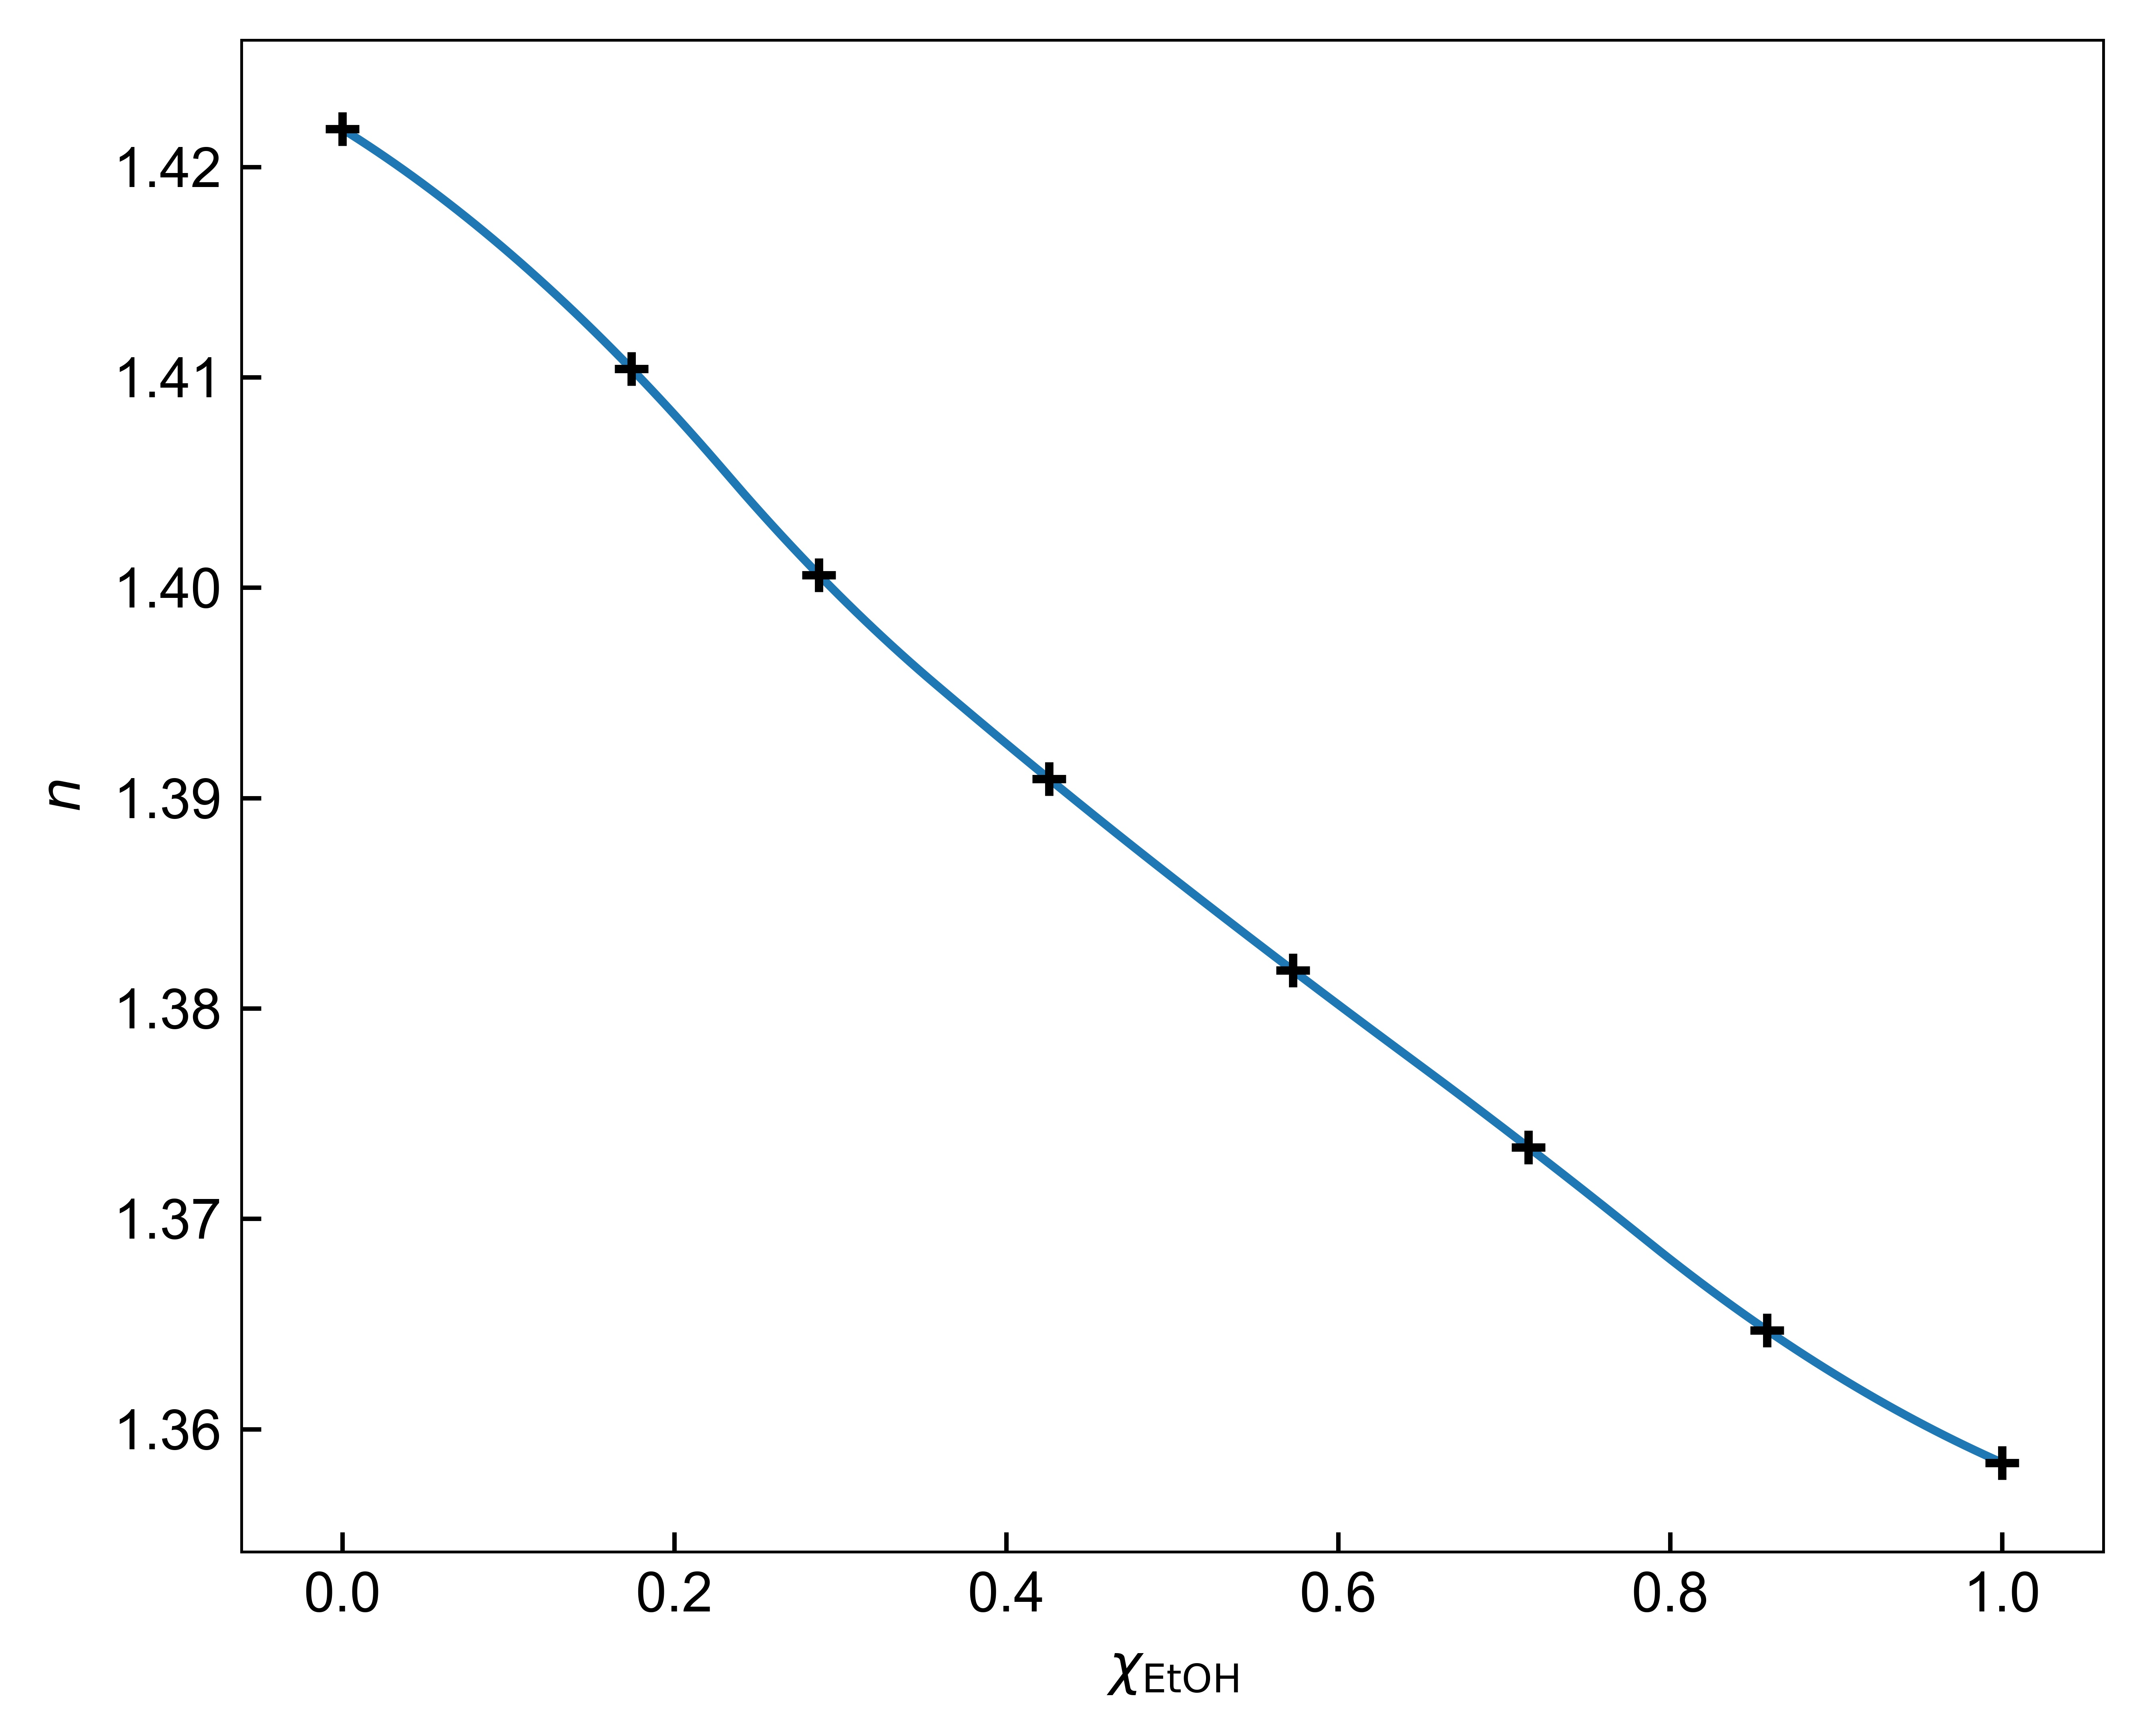
\includegraphics[width=0.75\textwidth]{1.jpg}
	\bicaption{加入第$1\sim 6$组$\rm KNO_{3}$体系$\Delta T-t$曲线}{$\Delta T-t$ curve with ${\rm KNO_{3}}$ sample $1\sim 6$ addition}
\end{figure}
\par

\vbox{}


 \subsection{数据处理结果与分析}
 \subsubsection{溶液浓度$n_{0}$的计算}
$\rm KNO_{3}$溶液的浓度$n_{0}$可由下式求算:
$$
n_{0}=\frac{n_{1}}{n_{2}}=\frac{\rho_{1}V_{1}/M_{1}}{m_{2}/M_{2}}=\frac{\rho_{1} V_{1} M_{2}}{m_{2} M_{1}}
$$
其中$n_{1}$、$M_{1}$分别为溶剂$\rm H_{2}O$的物质的量和摩尔质量,$M_{1}=18.016\ \ {\rm g\cdot mol^{-1}}$;$n_{2}$、$m_{2}$、$M_{2}$分别为溶质$\rm KNO_{3}$的物质的量、加入总质量和摩尔质量,$M_{2}=101.11\ \ {\rm g\cdot mol^{-1}}$;$V_{1}$为$500\ \ {\rm mL}$容量瓶定容后量取的去离子水体积,$V_{1}=500.0\ \ {\rm mL}$;$\rho_{1}$为$\rm H_{2}O$的密度;近似认为实验过程中去离子水的密度不变,查阅\textit{CRC Handbook of Chemistry and Physics}\citealp{crc}知室温$T=17.6\ \ {\rm ^{\circ}C}$下水的密度$\rho_{1}=998.68\ \ {\rm g\cdot L^{-1}}$;以加入第1组$\rm KNO_{3}$的数据为例,计算溶液浓度
$$
n_{0}=\frac{\rho_{1} V_{1} M_{2}}{m_{2} M_{1}}=\frac{ 500.0\ \ {\rm mL} \times 101.11\ \ {\rm g\cdot mol^{-1}} \times 998.68\ \ {\rm g\cdot L^{-1}}}{12.1238\ \ {\rm g} \times 18.016\ \ {\rm g\cdot mol^{-1}}}=231.1
$$
\par 
类似地,计算加入第2$\sim$6组$\rm KNO_{3}$后的溶液浓度。记$\Delta m$为加入每一组$\rm KNO_{3}$的质量,$m_{2}$为累计加入$\rm KNO_{3}$的总质量,各溶液浓度$n_{0}$计算结果如\textbf{表7}所示。
\begin{table}[h]
	\centering
	\zihao{5}
	\bicaption{$\rm KNO_{3}$溶液浓度$n_{0}$计算数据}{$\rm KNO_{3}$ solution concentration $n_{0}$ calculation data}
	\begin{tabular}{ccccc}
		\toprule
		编号 & $\Delta m/{\rm g}$ &  $m_{2}/{\rm g}$ & $n_{2}/{\rm mol}$ & $n_{0}$ \\
		\midrule
		1 & 12.1238 & 12.1238 & 0.11991 & 231.1 \\
		2 & 12.0312 & 24.1550 & 0.23890 & 116.0 \\
		3 & 12.0995 & 36.2545 & 0.35856 & 77.30 \\
		4 & 5.0135  & 41.2680 & 0.40815 & 67.91 \\
		5 & 6.0353  & 47.3033 & 0.46784 & 59.24 \\
		6 & 8.0435  & 55.3468 & 0.54739 & 50.63 \\
		\bottomrule
	\end{tabular}
\end{table}
\par


\subsubsection{体系吸热$Q$的计算}
从\textbf{图1(1)$\sim$(6)}中读取加入$\rm KNO_{3}$样品时体系初始温度$\Delta T_{1}$、加入$\rm KNO_{3}$后体系最低温度$\Delta T_{2}$、通电前(开始加热时)体系温度$\Delta T^{\prime}_{2}$、通电加热后体系最终温度$\Delta T^{\prime}_{1}$及通电加热时间$\Delta t$。注意到由于机械搅拌做功,停止加热后体系温度仍不断上升;为保证结果的一致性,使用python SciPy linregress分别作出通电加热过程和通电加热后$\Delta T-t$实验数据的拟合直线,读取两拟合直线交点对应的温度,即为$\Delta T^{\prime}_{1}$。需要说明的是,上述方法得到的$\Delta T^{\prime}_{1}$并未充分排除热交换等因素导致的误差,具体将在4.1.1予以讨论。\par 
加入第$1\sim 6$组$\rm KNO_{3}$后的体系吸热$Q$可由下式求算:
$$
Q=\frac{\Delta T_{2}-\Delta T_{1}}{\Delta T^{\prime}_{2}-\Delta T^{\prime}_{1}} \ \ I^{2}R \Delta t
$$
其中$R=9.76\ \ \Omega$为电阻丝阻值,$I=1.18\ \ {\rm A}$为加热电流,$\Delta t$为加热时间;以加入第1组$\rm KNO_{3}$的数据为例,计算体系吸热
$$
Q=\frac{\Delta T_{2}-\Delta T_{1}}{\Delta T^{\prime}_{2}-\Delta T^{\prime}_{1}} \ \ I^{2}R \Delta t=\frac{-1.974-0.003}{-1.963-0.198}\times (1.18\ \ {\rm A})^{2}\times 9.76\ \ \Omega\times 360\ \ {\rm s}=4.47\ \ {\rm kJ}
$$
\par 
类似地,计算加入$2\sim 6$组$\rm KNO_{3}$后的体系吸热$Q$。加入各组$\rm KNO_{3}$的体系吸热$Q$计算结果如\textbf{表8}所示。
\begin{table}[h]
	\centering
	\zihao{5}
	\bicaption{加入$\rm KNO_{3}$体系吸热$Q$计算数据}{System thermal effect $Q$ calculation data with $\rm KNO_{3}$ addition}
	\begin{tabular}{cccccccc}
		\toprule
		编号 & $n_{0}$ &  $\Delta T_{1}/{\rm ^{\circ}C}$ & $\Delta T_{2}/{\rm ^{\circ}C}$ & $\Delta T^{\prime}_{1}/{\rm ^{\circ}C}$ & $\Delta T^{\prime}_{2}/{\rm ^{\circ}C}$ & $\Delta t/{\rm s}$ & $ Q/{\rm kJ}$ \\
		\midrule
		1 & 231.1 & 0.003 & -1.974 & 0.199  & -1.963 & 360 & 4.47 \\
		2 & 116.0 & 0.008 & -1.849 & 0.059  & -1.838 & 315 & 4.19 \\
		3 & 77.30 & 0.008 & -1.766 & 0.061  & -1.760 & 300 & 3.97 \\
		4 & 67.91 & 0.008 & -0.699 & 0.119  & -0.693 & 135 & 1.60 \\
		5 & 59.24 & 0.008 & -0.821 & -0.003 & -0.819 & 135 & 1.86 \\
		6 & 50.63 & 0.007 & -1.081 & 0.024  & -1.074 & 180 & 2.42 \\
		\bottomrule
	\end{tabular}
\end{table}
\par

\subsubsection{溶液$Q_{s}$、$n_{0}$的计算及$Q_{s}-n_{0}$图}
根据\textbf{表7}数据,计算每次加入$\rm KNO_{3}$后体系总的热效应$\Sigma Q$。根据定义,积分溶解热$Q_{s}$可由下式求算:
$$
Q_{s}=\frac{\Sigma Q}{n_{2}}
$$
以加入第1组$\rm KNO_{3}$的数据为例,计算积分溶解热
$$
Q_{s}=\frac{\Sigma Q}{n_{2}}=\frac{4.47\ \ {\rm kJ}}{0.11991\ \ {\rm mol}}=37.3\ \ {\rm kJ\cdot mol^{-1}}
$$
计算加入各组$\rm KNO_{3}$的积分溶解热$Q_{s}$,结果如\textbf{表9}所示。
\begin{table}[h]
	\centering
	\zihao{5}
	\bicaption{加入$\rm KNO_{3}$体系吸热$Q$计算数据}{System thermal effect $Q$ calculation data with $\rm KNO_{3}$ addition}
	\begin{tabular}{cccccc}
		\toprule
		编号 & $n_{0}$ &  $n_{2}/{\rm mol}$ & $Q/{\rm kJ}$ & $ \Sigma Q/{\rm kJ}$ & $Q_{s}/{\rm kJ\cdot mol^{-1}}$ \\
		\midrule
		1 & 231.1 & 0.11991 & 4.47 & 4.47  & 37.3 \\
		2 & 116.0 & 0.23890 & 4.19 & 8.67  & 36.3 \\
		3 & 77.30 & 0.35856 & 3.97 & 12.64 & 35.2 \\
		4 & 67.91 & 0.40815 & 1.60 & 14.24 & 34.9 \\
		5 & 59.24 & 0.46784 & 1.86 & 16.10 & 34.4 \\
		6 & 50.63 & 0.54739 & 2.42 & 18.52 & 33.8 \\
		\bottomrule
	\end{tabular}
\end{table}
\par
作出$Q_{s}-n_{0}$散点图,并使用python SciPy optimize用经验方程
$$
Q_{s}=Q^{0}_{s}\frac{an_{0}}{1+an_{0}}
$$
进行拟合,得到$Q_{s}-n_{0}$拟合曲线,如\textbf{图2}所示。

\begin{figure}[h]
	\centering
	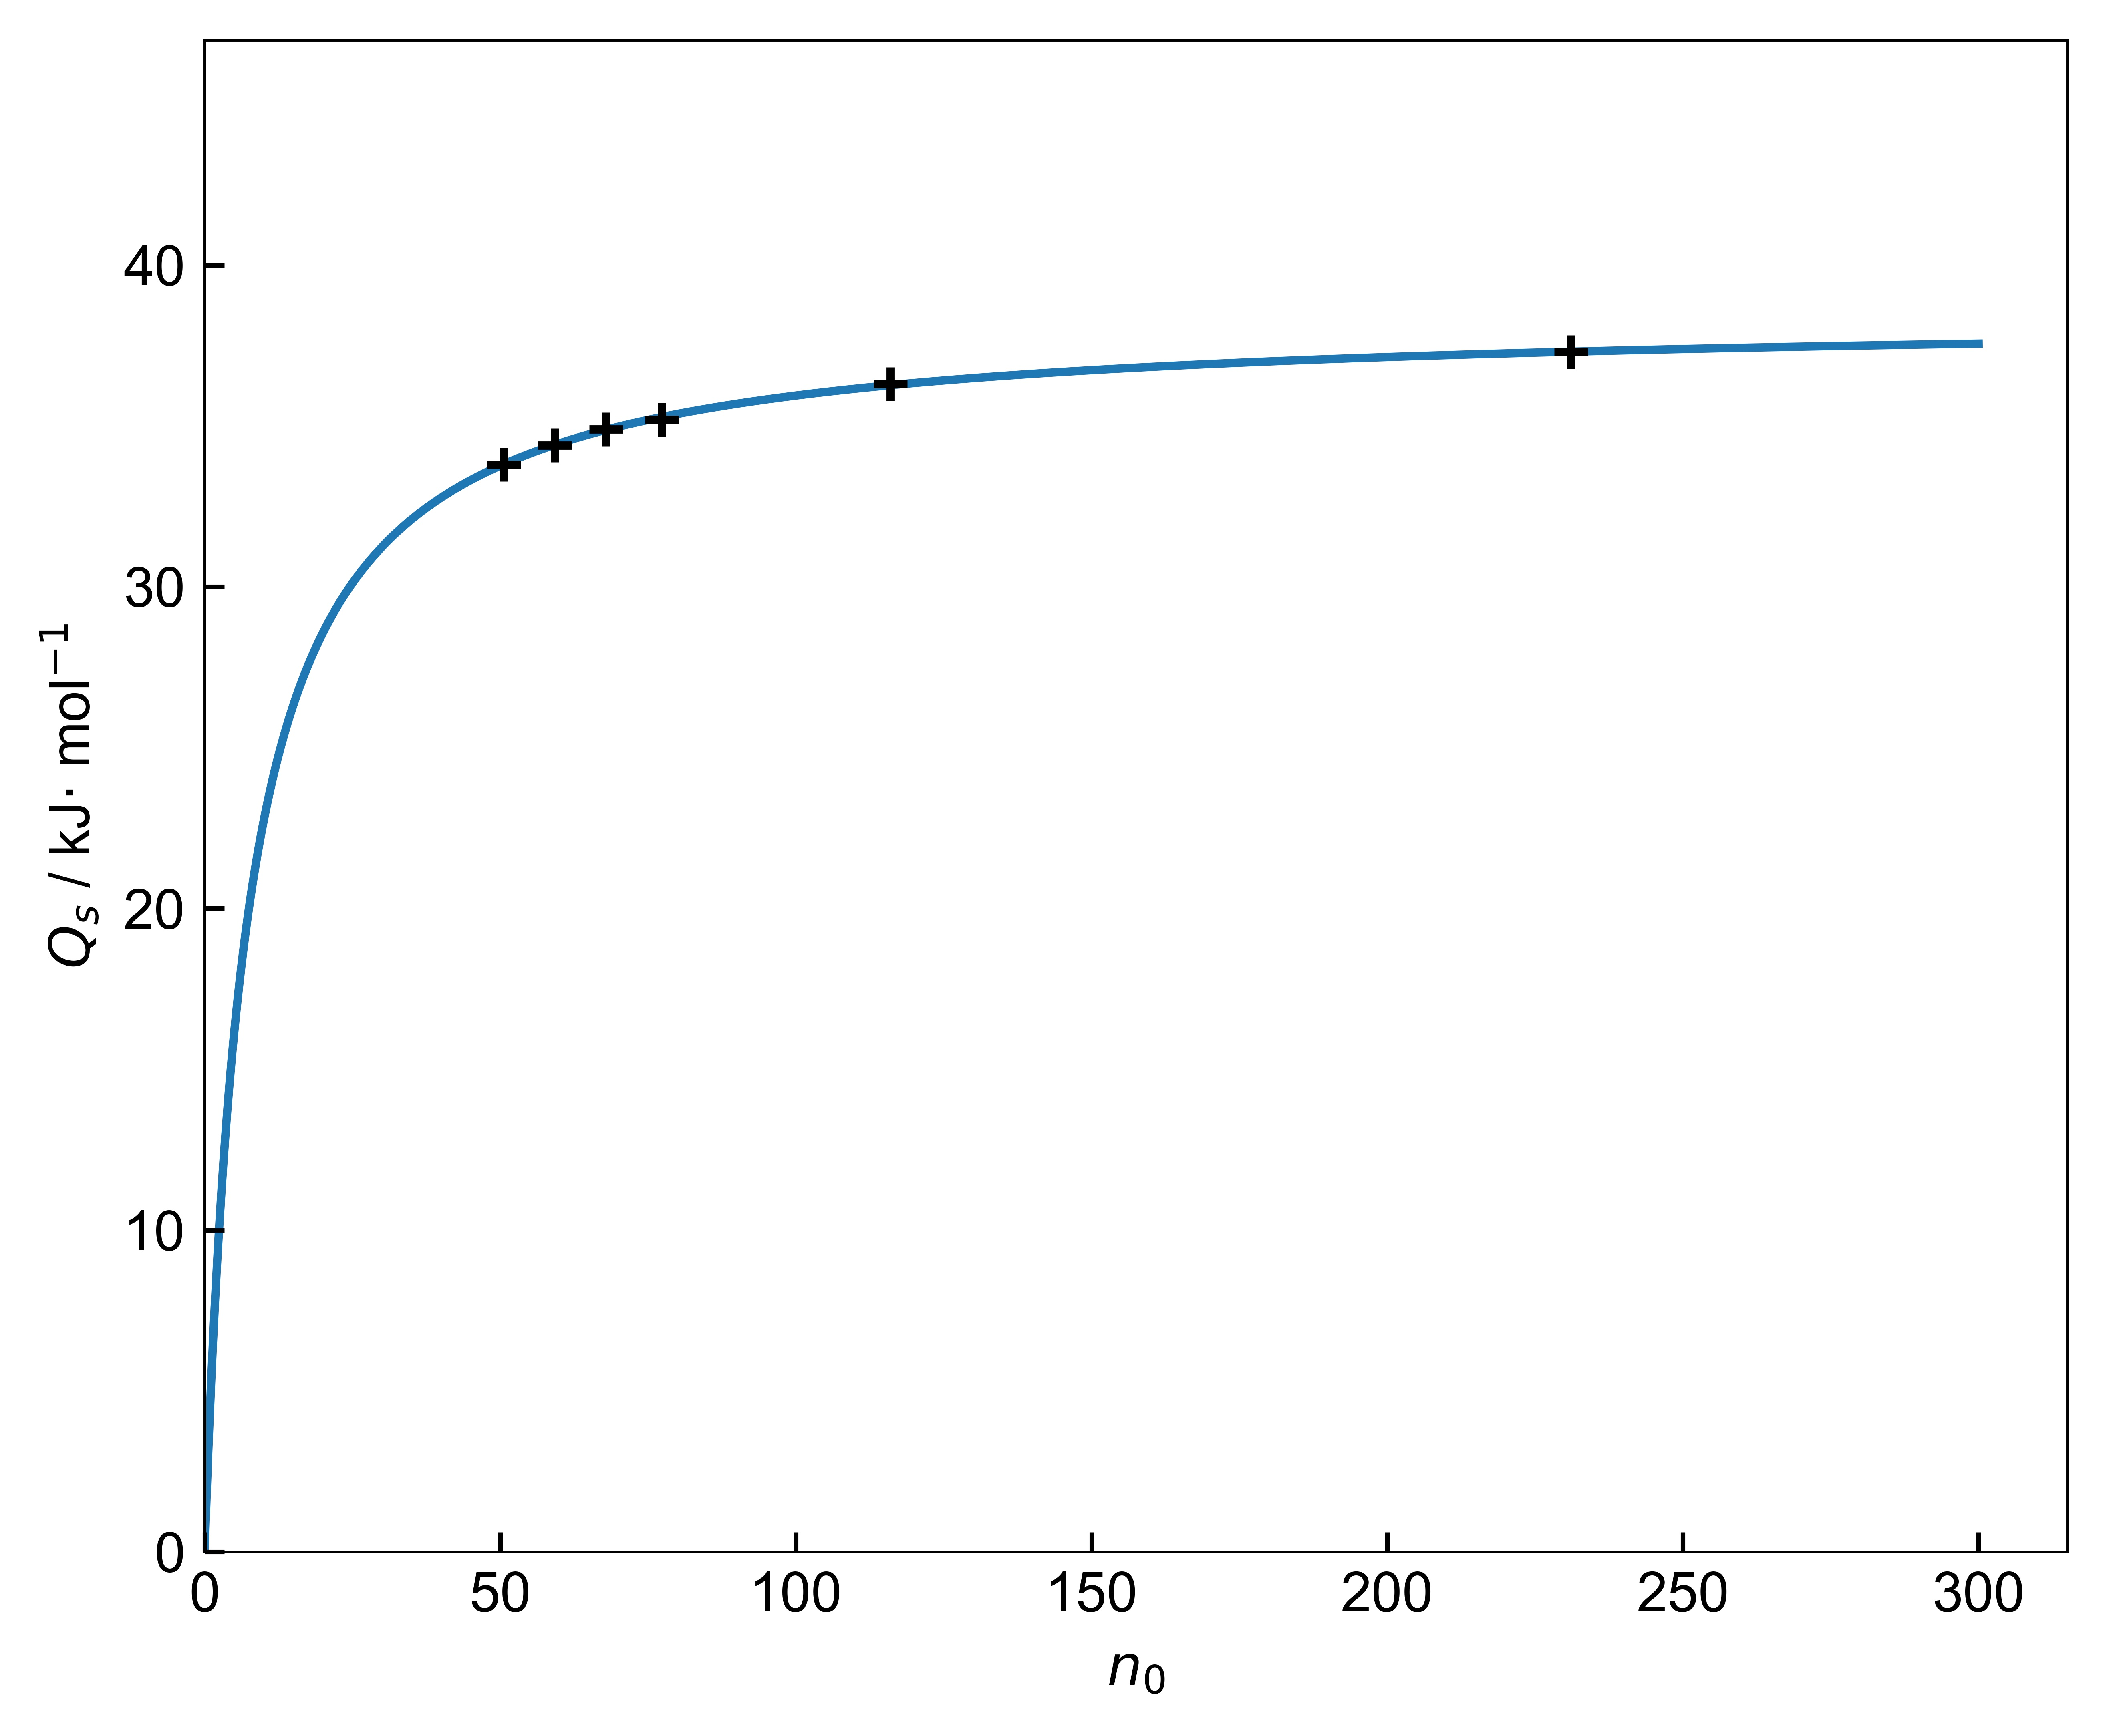
\includegraphics[width=0.60\textwidth]{2.jpg}
	\bicaption{$Q_{s}-n_{0}$图及拟合曲线}{$Q_{s}-n_{0}$ diagram and fitted curve}
\end{figure}
\par
拟合曲线的方程为
$$
Q_{s}/{\rm kJ\cdot mol^{-1}} = (38.42\pm 0.02)\times \frac{(0.145\pm 0.001)n_{0}}{1+(0.145\pm 0.001)n_{0}},\  \ R^{2}=0.99983
$$
即
$$
Q^{0}_{s}=(38.42\pm 0.02)\ \ {\rm kJ\cdot mol^{-1}}
$$
$$
a=0.145\pm 0.001
$$
拟合曲线$R^{2}=0.99983$,各数据点很好地落在$Q_{s}-n_{0}$拟合曲线上。
\subsubsection{微分冲淡热、微分溶解热及积分冲淡热的计算}
由微分方程推导得到
$$
Q_{s}=\diffp Q{n_{2}}[n_{1}]+n_{0}\diffp {Q_{s}}{n_{0}}[n_{2}]
$$
即为$Q_{s}-n_{0}$曲线上任意一点$(n_{0}, Q_{s})$处切线的方程,切线斜率即为微分冲淡热$\diffp {Q_{s}}{n_{0}}[n_{2}]$,截距即为微分溶解热$\diffp Q{n_{2}}[n_{1}]$,而积分冲淡热$Q_{d}$即为两浓度$n_{1}$、$n_{2}$ $(n_{2}>n_{1})$下积分溶解热$Q_{s}$之差,即
$$
Q_{d}=(Q_{s})_{n_{2}}-(Q_{s})_{n_{1}}
$$
\par 
由3.2.3知$Q_{s}-n_{0}$拟合曲线的方程为
$$
Q_{s} =Q^{0}_{s}\frac{an_{0}}{1+an_{0}}= 38.42\times \frac{0.145 n_{0}}{1+0.145 n_{0}}\ \ {\rm kJ\cdot mol^{-1}}
$$
故计算得到任意一点$(n_{0}, Q_{s})$处切线斜率即微分冲淡热为
$$
\diffp {Q_{s}}{n_{0}}[n_{2}]=\frac{Q^{0}_{s}a}{(1+an_{0})^{2}}=\frac{38.42\times 0.145}{(1+0.145n_{0})^{2}}\ \ {\rm kJ\cdot mol^{-1}}
$$
切线截距即微分溶解热为
$$
\diffp Q{n_{2}}[n_{1}]=\frac{Q^{0}_{s}a^{2}n^{2}_{0}}{(1+an_{0})^{2}}=\frac{38.42\times 0.145^{2} \times n^{2}_{0}}{(1+0.145n_{0})^{2}}\ \ {\rm kJ\cdot mol^{-1}}
$$
根据以上各式,分别计算$n_{0}=200$、$n_{0}=150$、$n_{0}=100$、$n_{0}=80$、$n_{0}=50$时的积分溶解热$Q_{s}$、微分冲淡热$\diffp {Q_{s}}{n_{0}}[n_{2}]$、微分溶解热$\diffp Q{n_{2}}[n_{1}]$,并根据相邻两组数据计算积分冲淡热$Q_{d}$,计算结果如\textbf{表10}所示。
\begin{table}[h]
	\centering
	\zihao{5}
	\bicaption{不同浓度$\rm KNO_{3}$溶解热相关计算数据}{Correlative calculation data of $\rm KNO_{3}$ dissolution heat of different concentration}
	\begin{tabular}{ccccc}
		\toprule
		$n_{0}$ &  $Q_{s}/{\rm kJ\cdot mol^{-1}}$ & $\diffp {Q_{s}}{n_{0}}[n_{2}]/{\rm kJ\cdot mol^{-1}}$ & $ \diffp Q{n_{2}}[n_{1}]/{\rm kJ\cdot mol^{-1}}$ & $Q_{d}/{\rm kJ\cdot mol^{-1}}$ \\
		\midrule
		200 & 37.14 & 0.00619 & 35.90 &      \\
		150 & 36.73 & 0.01076 & 35.12 & 0.41 \\
		100 & 35.94 & 0.02319 & 33.62 & 0.79 \\
		80  & 35.37 & 0.03509 & 32.56 & 0.57 \\
		50  & 33.76 & 0.08185 & 29.67 & 1.61 \\
		\bottomrule
	\end{tabular}
\end{table}
\par
根据\textbf{表10}可以看出,不同浓度$n_{0}$下均有
$$
Q_{s}\gg Q_{d}
$$
$$
\diffp Q{n_{2}}[n_{1}]\gg \diffp {Q_{s}}{n_{0}}[n_{2}]
$$
即$\rm KNO_{3}$溶解的热效应主要来自溶解热,冲淡热占比很小。

\vbox{}

 	\section{讨论与结论}
		\subsection{实验讨论}
 			\subsubsection{雷诺校正对实验误差的影响}
 			欲使溶解热得到准确测定,需要尽可能排除体系与外界的热交换(包括电磁搅拌引入机械功)的影响。而在3.2.2中,读取$\Delta T$时并未对以上因素进行修正,这引入了一定的实验误差。\par 
 			雷诺校正是常用的校正体系和环境热交换的方法,下面以加入第1组$\rm KNO_{3}$后体系$\Delta T-t$的相关数据为例,对测得温度进行雷诺校正,并依此估算体系与外界的热交换所引入的实验误差。考虑到$\rm KNO_{3}$溶解过程中,加入$\rm KNO_{3}$后温度迅速降至最低温度$\Delta T_{2}$,可以认为在$\rm KNO_{3}$溶解过程中体系与外界的热交换可以忽略不计,是否进行雷诺校正对$\Delta T_{1}$、$\Delta T_{2}$的测定影响不大;而电加热过程持续较长时间,雷诺校正对$\Delta T^{\prime}_{1}$、$\Delta T^{\prime}_{2}$的准确测定有着重要意义,因此对电加热过程的体系温度变化进行雷诺校正,如\textbf{图3}所示。
 			
 			\begin{figure}[h]
 				\centering
 				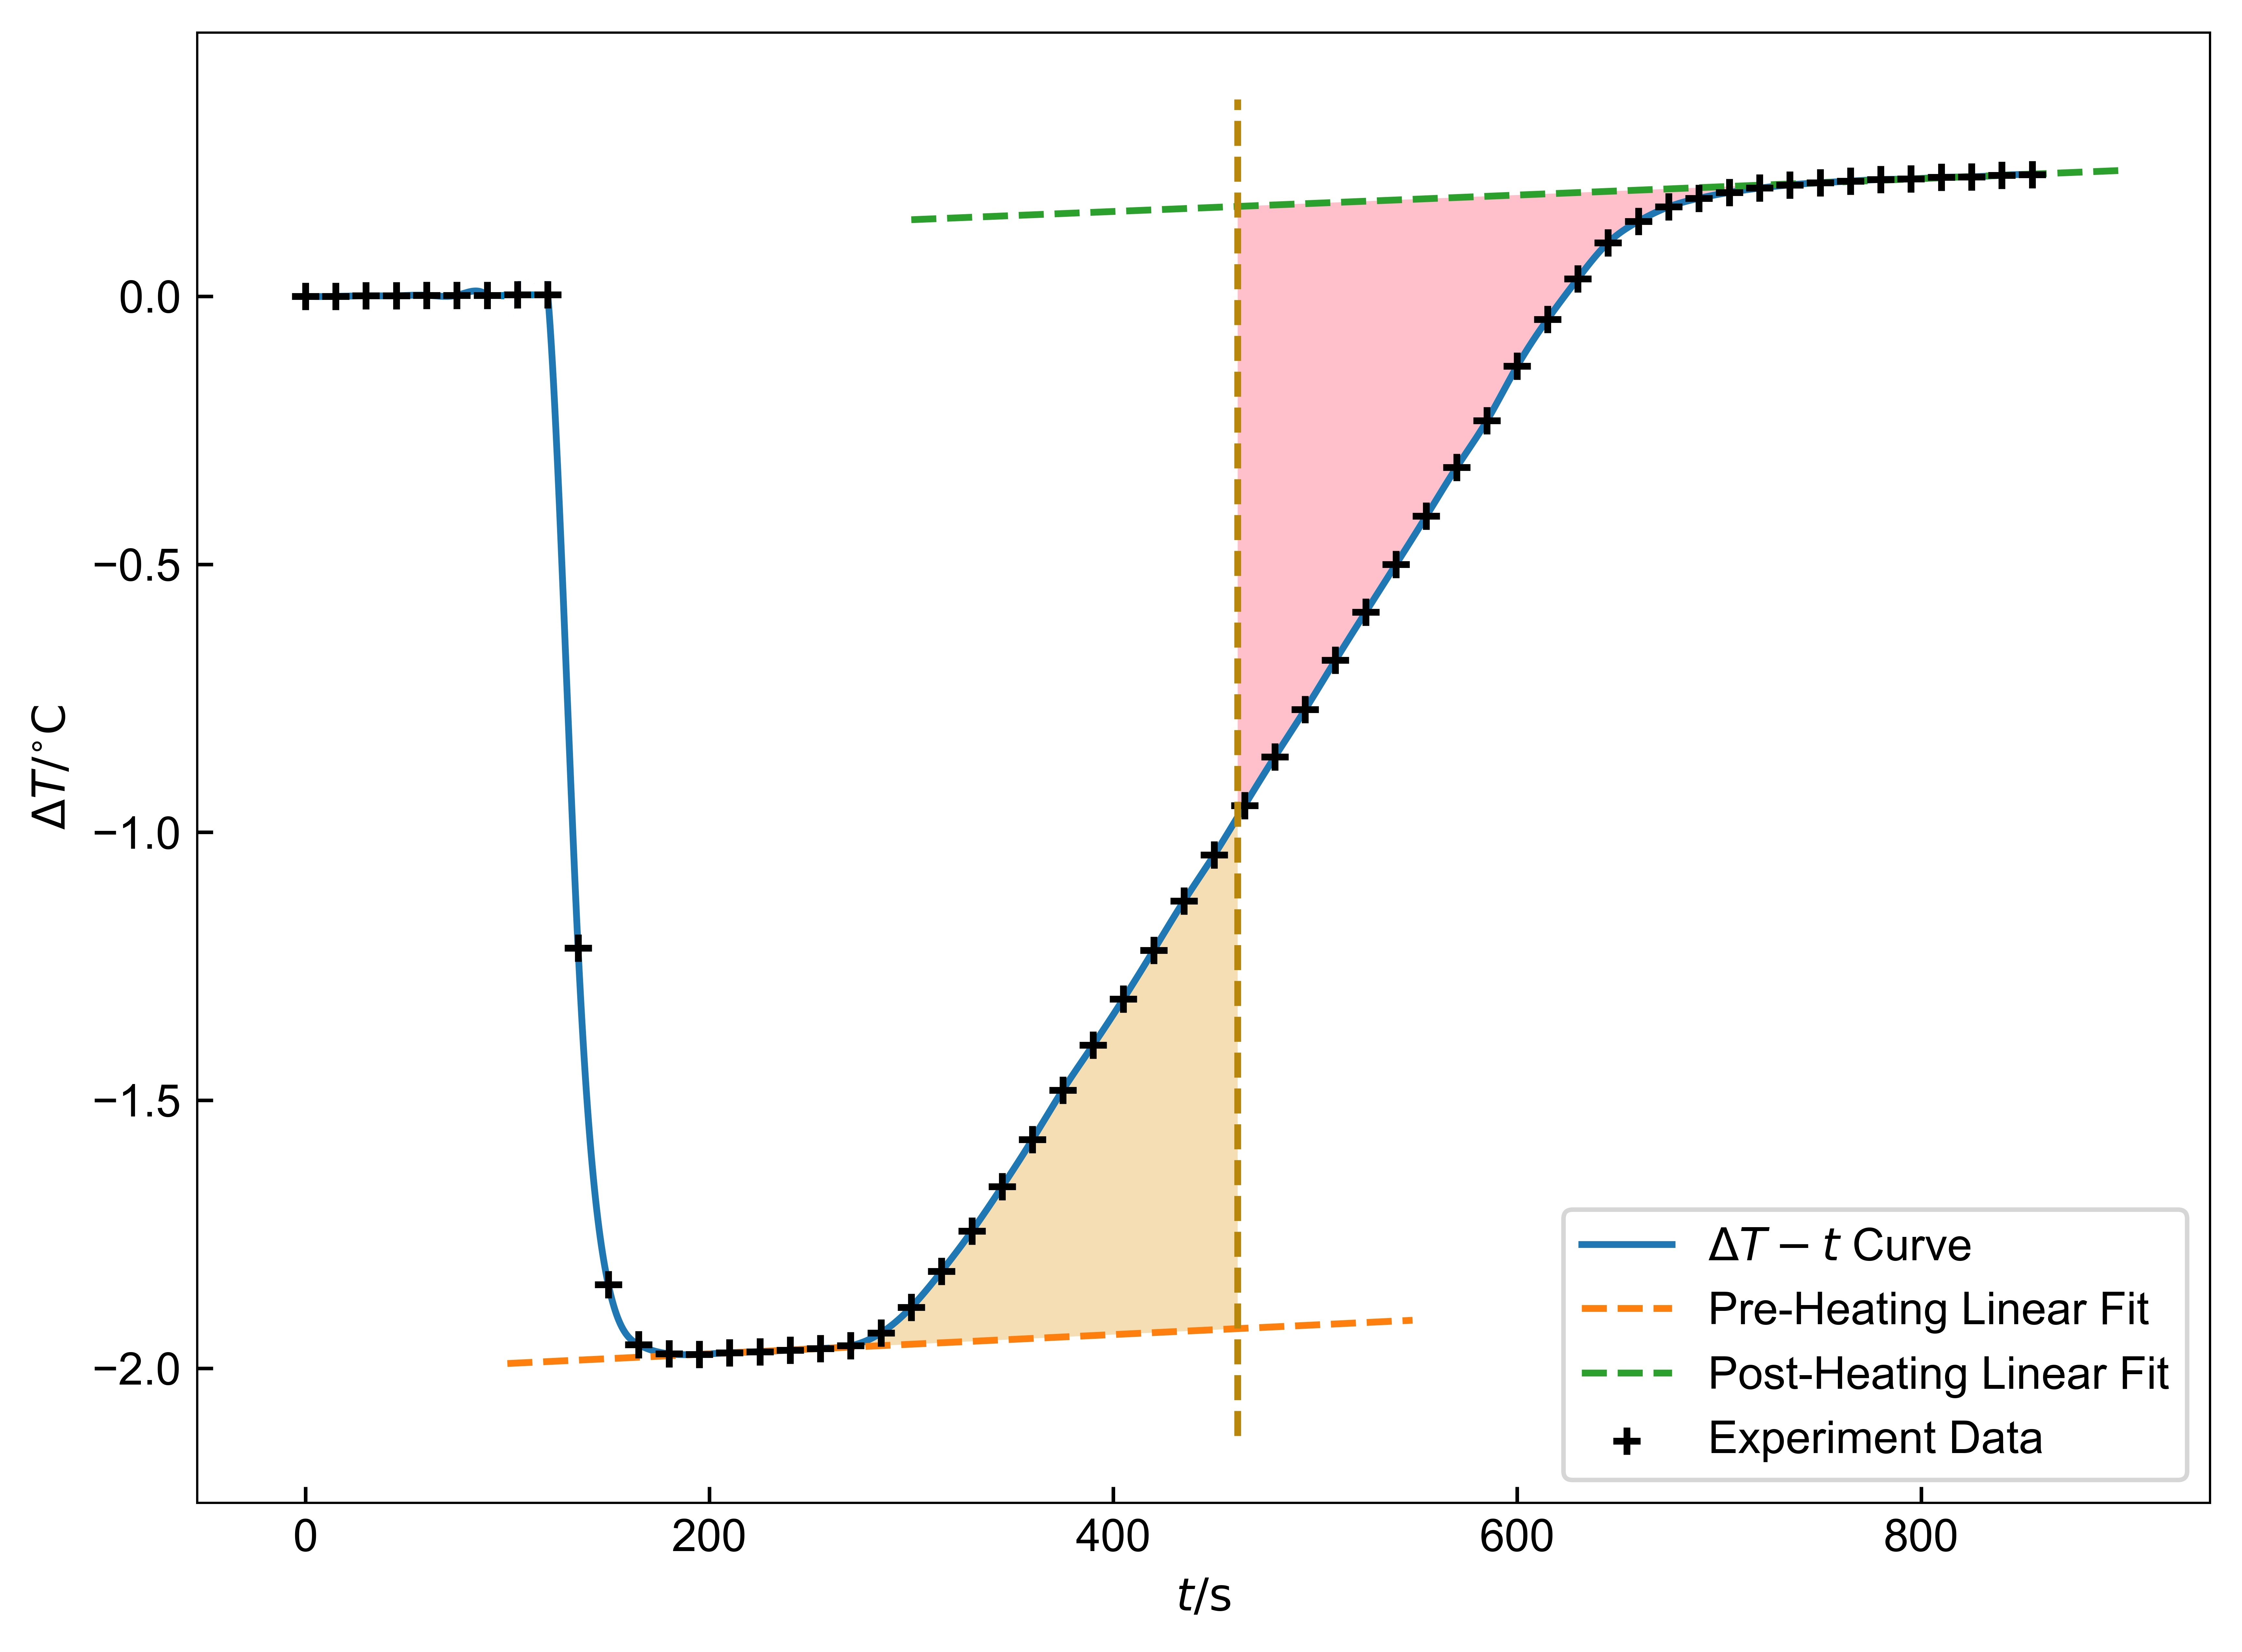
\includegraphics[width=0.65\textwidth]{3.jpg}
 				\bicaption{加入第1组$\rm KNO_{3}$体系$\Delta T-t$曲线及雷诺校正}{$\Delta T-t$ curve with $\rm KNO_{3}$ sample 1 addition and Renolds correction}
 			\end{figure}
 			\par
 			
 			根据\textbf{图3},读出经雷诺校正后的$\Delta T^{\prime}_{1}=-1.926\ \ {\rm K}$,$\Delta T^{\prime}_{2}=0.168\ \ {\rm K}$,依此计算体系吸热
 			$$
 			Q^{\prime}=\frac{\Delta T_{2}-\Delta T_{1}}{\Delta T^{\prime}_{2}-\Delta T^{\prime}_{1}} \ \ I^{2}R \Delta t=\frac{-1.974-0.003}{-1.926-0.168}\times (1.18\ \ {\rm A})^{2}\times 9.76\ \ \Omega\times 360\ \ {\rm s}=4.62\ \ {\rm kJ}
 			$$
 			对比3.2.2未经雷诺校正下计算得到的体系吸热$Q=4.47\ \ {\rm kJ}$,可以近似认为体系与外界的热交换导致的实验误差
 			$$
 			\Delta Q=Q-Q^{\prime}=-0.15\ \ {\rm kJ}
 			$$
 			相对误差
 			$$
 			\xi=\frac{\Delta Q}{Q^{\prime}}\times100\%=-3.2\%
 			$$
 			可见体系与外界的热交换对$Q$的测定误差有着相当大的贡献。考虑到$Q$的测定误差直接导致$Q_{s}$、$\diffp {Q_{s}}{n_{0}}[n_{2}]$、$\diffp {Q}{n_{2}}[n_{1}]$、$Q_{d}$的同等量级的相对误差,故使用雷诺校正对电加热过程体系温度变化进行修正能够显著减小实验误差。
 			\subsubsection{误差分析:$\rm KNO_{3}$固体洒落及残留引入实验误差}
 			在实验过程中,通过漏斗向溶液中加入第1组$\rm KNO_{3}$样品时,由于操作不够熟练,有少量$\rm KNO_{3}$固体洒落,并且有少量$\rm KNO_{3}$粉末残留在称量纸上。估算洒落及残留的$\rm KNO_{3}$固体质量约为$\Delta m=0.1000\ \ {\rm g}$,则实际加入的$\rm KNO_{3}$质量为
 			$$\Delta m^{\prime}_{1}=\Delta m_{1}-\Delta m=12.0238\ \ {\rm g}$$
 			依此计算
 			$$
 			Q^{\prime}_{s}=\frac{Q}{n^{\prime}_{2}}=37.6\ \ {\rm kJ\cdot mol^{-1}}
 			$$
 			相对误差
 			$$
 			\xi=\frac{Q_{s}-Q^{\prime}_{s}}{Q^{\prime}_{s}}\times 100\%=-0.80\%
 			$$
 			故$\rm KNO_{3}$固体洒落及残留导致$Q_{s}$测量值偏小,并为后续数据的计算引入误差,但相对误差$\xi$的大小小于体系与外界的热交换带来的相对误差,故不是主要的影响因素。\par 
 			除以上误差外,实验中$\rm KNO_{3}$固体吸潮、经验方程拟合误差、电阻丝阻值波动等也是可能的误差来源,限于篇幅不作一一讨论。 	
		
 			
 		



 	 \subsection{实验结论}
 	 本实验通过电热补偿法测定了累次加入的$\rm KNO_{3}$溶解过程的热效应$Q$,计算了积分溶解热$Q_{s}$,作$Q_{s}-n_{0}$图并用经验公式进行拟合,作切线得到$\rm KNO_{3}$的微分冲淡热$\diffp  {Q_{s}}{n_{0}}[n_{2}]$约为$0.006\sim 0.08\ \ {\rm kJ\cdot mol^{-1}}$,微分溶解热$\diffp  {Q}{n_{2}}[n_{1}]$约为$30\sim 36\ \ {\rm kJ\cdot mol^{-1}}$,积分冲淡热$Q_{d}$约为$0.4\sim 1.6\ \ {\rm kJ\cdot mol^{-1}}$,根据以上数据可以判断$\rm KNO_{3}$溶解的热效应主要来自溶解热,冲淡热占比很小。\par 
 	 本文讨论了实验误差的大小及来源、雷诺校正对实验误差的影响。经计算,体系与外界的热交换是主要的误差来源,对$Q$的测定带来$\xi=-3.2\%$的相对误差;此外,$\rm KNO_{3}$固体洒落及残留、$\rm KNO_{3}$固体吸潮、经验方程拟合误差、电阻丝阻值波动等也是次要的可能误差来源。


 

   

\vbox{}

\bibliographystyle{achemso}
\bibliography{b}



\end{document}